\documentclass[12pt,a4paper]{article}
\usepackage[utf8]{inputenc}
\usepackage[magyar]{babel}
\usepackage[T1]{fontenc}
\usepackage{amsmath}
\usepackage{amsfonts}
\usepackage{amssymb}
\usepackage{graphicx}
\begin{document}

GTLib feladatok gyakorlása

\begin{itemize}

\item Számoljuk ki egy szöveges állományban elhelyezett egész számok összegét!
\item Számoljuk ki egy természetes szám faktoriálisát!
\item Válogassuk ki egy szöveges állományban elhelyezett egész számok közül a párosakat!
\item Melyik egy tömb első olyan eleme, amelyik először ismétlődik?
\item Ki a kurzus legjobb hallgatója? A hallgatók nevét és a kapott részeredményeiket (0 és 5
közötti jegyek) egy-egy sorban adtuk meg egy szöveges állományban.
\item Ki a kurzus legjobb hallgatója? A hallgatók nevét és részeredményét (0 és 5 közötti jegy) egy-
egy sorban, ugyanazon nevű hallgató sorai közvetlenül egymás után adtuk meg egy szöveges
állományban.

\end{itemize}

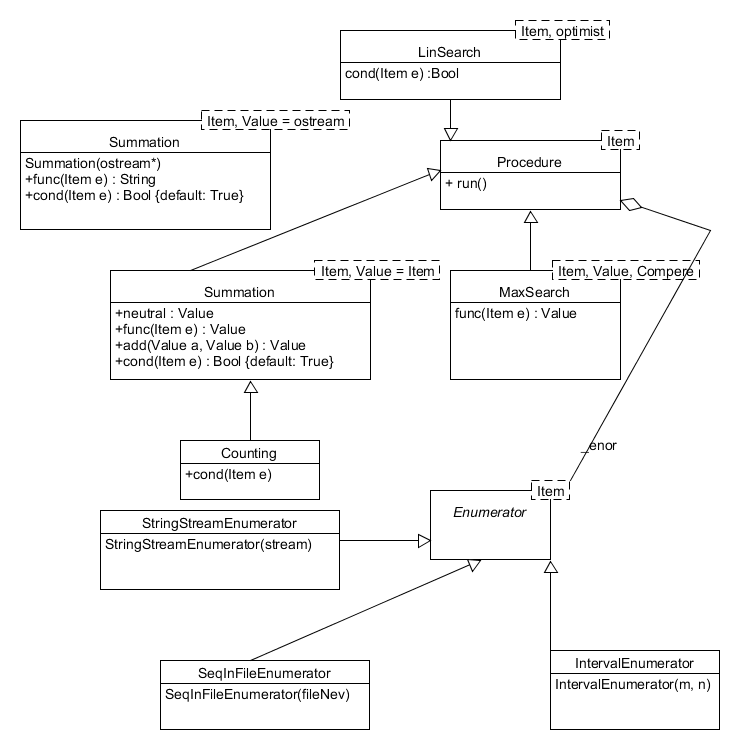
\includegraphics[scale=0.6]{gtlib_uml.png}

\end{document}